%%=========================================
\section[Eksperimenter \& Resultater]{Eksperimenter \& Resultater}
%%=========================================\\
\subsection{Evalueringsstrategier}
For at en hypotese skal bevises gjennom den vitenskapelige metode kreves det logisk argumentasjon, empiriske bevis og at eksperimentet er reproduserbart. Alle hypotesene jeg har dannet utforskes i dette kapitellet med argumentasjon, men de empiriske bevisene vil mangle i noen tilfeller. Dette er rett og slett fordi det vil kreve mer tid og utførelse av brukertesting for å bevise disse hypotesene. Gestegjenkjennelsen vil evalueres av den prosentvise korrekte klassifiseringen. Den vil også evalueres etter hvor mange gester det lærte systemet kan skille mellom, mot hvor mange som kan eksplisitt programmeres. Dette gjelder hypotesene 1 og 3. Hypotesene 2 og 4 lener seg hovedsaklig på argumentasjon.\\

\subsection{Eksperimentsutførelse}
\subsubsection*{Gestegjenkjennelse gjennom fotodioder}
Dersom man ønsker å tilby styringsmuligheter på en eller flere vegger i et hus kan enkle gestesensorer benyttes i steden for et panel av knapper og dimmere. I det forrige kapitellet så vi at den aktuelle sensoren er på størrelse med et knappenålshode. Gode produktdesignere vil med dette utgangspunktet kunne kan lage et produkt som enten forsvinner inn i hjemmiljøet, eller et som synes tydelig, men er praktisk og estetisk. Sensoren merker at en hånd eller et annet objekt befinner seg foran den ved å sende ut et svakt infrarødt signal som reflekteres. Signalet detekteres dersom signalet er tilstrekkelig sterkt nok når det returnerer. Dette vil bare skje dersom objektet er opptil 20 cm unna sensoren. Gester forstås dermed kun når de utføres rett foran sensoren.

I motsetning til forståelse av gester gjennom bruk av kameraer er dette altså en langt mindre påtrengende måte å interagere med brukerne. De kan være sikre på å verken være overvåket eller at personvernet deres på noen måte krenkes. Gestesensoren fungerer som en multifunksjonell knapp.\\
\begin{wrapfigure}{r}{0.4\textwidth}
    \vspace{-20pt}
  \begin{center}
    \includegraphics[width=0.35\textwidth]{fig/swipe-l-r}
  \end{center}
  \vspace{-20pt}
  \caption{Gest: brukeren sveiper hånd mot venstre}
  \label{fig:gest}
  \vspace{-7pt}
\end{wrapfigure}
Figur \ref{fig:gest} viser en typisk gest der brukeren sveiper hånda foran sensoren som befinner seg på veggen. Kanskje denne sveipende bevegelsen foran denne sensoren betyr å skru av lyset i rommet sensoren befinner seg i. Eller kanskje gesten betyr å skru på radioen, låse opp en dør, lukke gardinene eller starte kaffemaskinen. Det er ingen begrensning på hva en enkelt gest aktiverer i form av funksjonalitet.

Når en gest utføres må enten rådataene fra sensoren eller en forståelse av dataene sendes til et system som har ansvaret for å styre hjemmet. Sensoren må være knyttet til en mikrokontroller eller tilsvarende som har ansvaret for å sende dataene videre. Dette kan enten være gjennom kabel eller trådløst. Det er mulig å programmere en mikrokontroller til å skille mellom sensordataene og forstå seks ulike gester\footnote{https://github.com/sparkfun/APDS-9960\_RGB\_and\_Gesture\_Sensor}. Dette er i seg selv bra og betyr at en enkelt sensor kan fungere som en knapp med seks forskjellige innstillinger. Hvis man også utnytter at kombinasjonen av flere gester etter hverandre kan bety egne kommandoer er styringsmulighetene mange. Det finnes et alternativ til å programmere hva de ulike dataene skal tolkes som. Alternativet er å sende rådataene til en kraftigere maskin som kan benytte den spennende teknikken kjent som maskinlæring til å forstå potensielt enda flere ulike gester.

Jeg kjørte Python-scriptet \emph{process-data.py} for å åpne tilkoblingen til den serielle porten mikrokontrolleren sender data til. Porten åpnes periodisk i noen sekunder og ber om at en gest utføres. Jeg gjennomførte 50 utførelser av hver av de 10 gestene (se figur \ref{fig:gester}), for totalt 500 datapunkter. I illustrasjonene indikerer en enkelt pil et rolig sveip over sensoren. Tre piler indikerer en større hastighet. Dataene fra hver gest ble lagret i individuelle filer i kommaseparert format. Med dataene for hver gest lagret i forskjellige filer kan disse kombineres slik man ønsker, for å trene systemet til å skille mellom 2,3, eller opp til 10 gester. 

Maskinlæring handler om å la maskinen lære fra data. Dette kan enten være et forsøk på å finne ukjente sammenhenger i dataene den mates med eller det kan være å lære seg sammenhenger mellom dataeksempler og klasser. Det er dette sistnevnte scenariet vi er interessert i. Vi kan mate maskinen med data fra en gest og samtidig gi informasjon om at dataene maskinen akkurat fikk betyr "sveip til høyre". Dermed kan maskinen forsøke å danne en optimal kobling mellom dataene som kom inn da vi sveipet til høyre og informerte om at disse dataene hørte til klassen "sveip til høyre". Med tilstrekkelig treningseksempler fra de ulike gestene skal maskinen kunne lære seg forskjellene mellom dem. Dermed vil den være i stand til å gjette riktig når en av de 10 gestene utføres senere. Prototypen jeg har utviklet er trent med 50 ulike dataeksempler på hver av de 10 ulike gestene.
\begin{figure}[h]
\begin{subfigure}{0.23\textwidth}
\includegraphics[width=3cm, height=3cm]{fig/swipe-r-l}
\caption{Sveip til høyre.}
\label{fig:sveip-}
\end{subfigure} 
\begin{subfigure}{0.23\textwidth}
\includegraphics[width=3cm, height=3cm]{fig/flick-l-r} 
\caption{Flikk til høyre.}
\label{fig:flikk-h}
\end{subfigure}
\begin{subfigure}{0.23\textwidth}
\includegraphics[width=3cm, height=3cm]{fig/swipe-r-l}
\caption{Sveip til venstre.}
\label{fig:sveip-v}
\end{subfigure} 
\begin{subfigure}{0.23\textwidth}
\includegraphics[width=3cm, height=3cm]{fig/flick-l-r}
\caption{Flikk til venstre.}
\label{fig:flikk-v}
\end{subfigure}
\begin{subfigure}{0.23\textwidth}
\includegraphics[width=3cm, height=3cm]{fig/swipe-d-u}
\caption{Sveip opp.}
\label{fig:sveip-opp}
\end{subfigure}
\begin{subfigure}{0.23\textwidth}
\includegraphics[width=3cm, height=3cm]{fig/flick-d-u}
\caption{Flikk opp.}
\label{fig:flikk-opp}
\end{subfigure}
\begin{subfigure}{0.23\textwidth}
\includegraphics[width=3cm, height=3cm]{fig/swipe-u-d}
\caption{Sveip ned.}
\label{fig:sveip-ned}
\end{subfigure}
\begin{subfigure}{0.23\textwidth}
\includegraphics[width=3cm, height=3cm]{fig/flick-u-d}
\caption{Flikk ned.}
\label{fig:flikk-ned}
\end{subfigure}
\begin{subfigure}{0.25\textwidth}
\includegraphics[width=3cm, height=3cm]{fig/near-far}
\caption{Nær - fjern.}
\label{fig:n-f}
\end{subfigure}
\begin{subfigure}{0.23\textwidth}
\includegraphics[width=3cm, height=3cm]{fig/far-near}
\caption{Fjern - nær.}
\label{fig:f-n}
\end{subfigure}
\caption{De 10 ulike gestene}
\label{fig:gester}
\end{figure}
Python-scriptet \emph{learning.py} utfører maskinlæringen. De lagrede dataene  lastes inn og de aktuelle klassene opprettes. Jeg splittet så dataene i et treningssett og et testsett. Splittingen var 75\% til trening og 25\% til testing. Dette er et viktig steg i prosessen for å ikke overspesialisere modellen til dataene. Dersom man trener algoritmen på hele datasettet og så tester på det samme settet, er det en sjanse for at modellen er overtilpasset. Man ønsker å finne den underliggende sammenhengen i dataene. Man ønsker ikke å danne en modell som perfekt representerer treningsdataene, men som ikke vil håndtere nye data godt. Hver modell blir trent og testet 100 ganger med et tilfeldig utgangspunkt hver gang, og sluttresultatet er et gjennomsnitt av disse 100 utførelsene.

\subsubsection*{Multimodal interaksjon gjennom tale og gester}
Mennesker i mellom kommuniserer i hovedsak med tale og det er forsket mye på å få datamaskiner til å forstå og bruke denne naturlige kommunikasjonsformen. Det er liten tvil om at det er en stor drøm for mange å ha en kontinuerlig samtale med datamaskinen. I et smart hjem kunne det vært hendig å spørre om statusoppdateringer om hjemmet, benytte tale for å få hjelp fra systemet til arbeid eller hobbyer, og gjøre oppslag etter matoppskrifter og værutsikter.

Så la oss fokusere på å bruke tale til det folk bruker tale til, nemlig å gi kommandoer og å stille spørsmål. Tale har først om fremst sin plass som \emph{kommunikasjonsprogramvare}. Tale kan også ha en begrenset nytte i forbindelse med læring; som å få faktasvar på tilstanden til hjemmet, eller for å lære om været for de neste dagene. Men for å bedrive dyp og god læring kreves det en aktiv utforskning. Vi lærer best ved å peke på ting, justere dem, holde dem i hendene og ved å ha muligheten til å bevege oss rundt dem. Tale virker upassende for denne typen aktiv utforskning. Når det gjelder programvare for å \emph{skape} virker det også som om tale kommer til kort. Jeg kan forestille meg at det i framtiden blir laget verktøy der brukeren forteller datamaskinen hva som skal gjøres for å lage noe. Men arbeid som involverer en evolusjon av produktet, som kunst eller ingeniørvirksomhet, er vanskelig å beskrive. Disse tingene skapes gradvis og vi manipulerer dem best med hendene våre. For meg fremstår tale hovedsaklig som en effektiv og naturlig interaksjonsform når det gjelder å gi enkle kommandoer, å hente informasjon eller å kommunisere med andre mennesker.

Dagens kommersielle løsninger, fra Google, Apple og andre, benytter seg av avanserte systemer for å forstå kontinuerlig tale. Med optimaliserte algoritmer og tilstrekkelig datakraft tilbyr disse aktørene talegjenkjenning med en svært høy grad av korrekthet. Men for å benytte tjenestene må talen som oppfattes av brukerens mikrofon sendes til kraftige maskiner på andre siden av kloden. Der prosesseres dataene, talen forstås og resultatet returneres. Det kan være vanskelig for disse systemene å garantere en god responstid. Dersom det tar flere sekunder før et resultat returneres vil nytteverdien til talegjenkjenning raskt minke. Umiddelbar respons vil være langt mer attraktivt. Denne tilnærmingen til talegjenkjenning har også problemer rundt bevarelse av personvernet. I et hvert tilfelle hvor data forsvinner ut av brukerens kontroll kan det være problemer. Det kan tenkes at taledata til tider inneholder sensitiv informasjon, som kalenderinformasjon, søkeord, eller tilstand i hjemmet. Og dersom informasjon om hjemmets alarmsystem eller status på beboere og låste dører forsvinner ut av hjemmet er dette en direkte sikkerhetsrisiko. En kjeltring, ute etter gjenstander eller identiteter, kan sitte på utsiden av hjemmet og få tilgang til sensitive data om hjemmet og dets beboere.

Samsung tilbyr både tale- og gestekontroll på sine nyere Smart-TV-er. En nærmere kikk på deres "global privacy policy" skapte i år oppstyr i media. Samsung tilsier seg retten til å lagre tale- og video-data for å forbedre tjenesten, samt å gi den videre til visse tredjepartier\footnote{\url{https://www.samsung.com/uk/info/privacy-SmartTV.html?CID=AFL-hq-mul-0813-11000170}}. Brukere har naturligvis vist misnøye med at alt de sier i stua kan bli tatt opp og sendt til tredjeparter. Samsung har advart brukeren om å diskutere personlig informasjon foran disse Smart-TV-ene. Personvernsbevisste brukere må altså passe på hva som blir sagt i sin egen stue.

Det kan se ut som det hadde vært optimalt å holde talegjenkjenningsprosessen lokal, og dermed unngå både treg responstid og mulig krenking av personvern. Er dette mulig i dag? Moderne telefoner, tv-er og andre enheter blir stadig kraftigere, men de er langt unna supercomputerene som for eksempel kjører Google's talegjenkjenning. Med flere prosessorkjerner vil ytelsen igjen øke i framtiden, men full bruk av disse trekker kraftig på batteriet.

Egenskapene jeg omtalte i \ref{ch:multimodalimpl} gjør Pocketsphinx til et interessant valg som kommunikasjonsprogramvare for smarte hjem. Problemdomenet vårt tilsier at vi ønsker et system som gjenkjenner et titalls kommandoer i reelltid. Det virker derfor ikke som det er nødvendig å knytte forståelsen opp mot internettet og sende taledata ut i verden. Vi kan unngå problemene med personvern, som Samsung og andre styrer med, ved å holde alle data lokalt. Ved å benytte et begrenset vokabular ofrer vi den kontinuerlige og mer naturlig talen. Til gjengjeld får vi en garantert bevarelse av personvernet.

I \ref{ch:multimodalimpl} nevnte jeg hvordan de fleste kommersielle produktene håndtere problemet med kontinuerlig lytting ved å benytte et aktiveringsord. Det finnes andre løsninger på dette problemet. Et avansert, men elegant, alternativ er å benytte stemmegjenkjenning. Her forstår systemet hvem som taler basert på talerens unike vokaltrakt. Systemet kan dermed programmeres til å kun godta kommandoer fra gjenkjente og klarerte brukere. En enklere løsning er å tilby talegjenkjenning i begrensede områder av hjemmet.
\begin{wrapfigure}{r}{0.4\textwidth}
    \vspace{-20pt}
  \begin{center}
    \includegraphics[width=0.35\textwidth]{fig/dictionary}
  \end{center}
  \vspace{-20pt}
  \caption{Vokabular}
  \label{fig:vokabular}
  \vspace{-7pt}
\end{wrapfigure}
For eksempel er det vanlig å tilbringe tiden alene på badet, så her kunne det vært aktuelt å la systemet lytte kontinuerlig da eventuell tale sannsynligvis vil være kommandoer til hjemmet. Jeg foreslår i dette eksperimentet å tilby kommandoutførelse gjennom tale kun dersom det også følger med en gest. Dette betyr at brukeren må stå foran enheten for å styre hjemmet. Enten kan en gest aktivere lyttingen, eller hjemmet kan lytte kontinuerlig, men kommandoer blir kun aktivert dersom en gest også utføres.

Pocketsphinx trenger et vokabular slik at den kan knytte taledata til ord og setninger. Man skriver en liste med setninger eller enkeltord man ønsker at systemet skal forstå. Deretter kan man benytte et språkmodell-verktøy til å få laget en språkmodell og et vokabular. Jeg har laget en ordliste med 38 elementer.

Jeg har først valgt å ta med substantiver; steder og ting i hjemmet, som "kitchen", "bedroom", "dishwasher" og "radio". Det er også andre substantiver som beskriver ting eller egenskaper ved mange av rommene eller apparatene: "lights", "temperature", "blinds", "curtains", "volume" og "power". Til sist er det med verb og preposisjoner, som "on", "up", "start", "increase" og "lock". Med et slikt vokabular kan brukeren potensielt styre det smarte hjemmet med en stor grad av kontroll.

Figur \ref{fig:vokabular} viser det resulterende vokabularet etter at verktøyet har prosessert en liste med ord. Vi ser at verktøyet forstår ordene som engelsk og tilfører data om engelsk uttale til listen. I noen tilfeller, som for "TV", er det flere alternative uttalser. Jeg skrev inn "TV" i ordlisten, og verktøyet har laget en forståelse for både "TV" og "television".

Vi har allerede pekt på problemene med å kontinuerlig lytte etter tale. Dersom systemet er slik at tale og gester må kombineres for effekt kan tale benyttes for å peke ut substantivet, eller hva som skal opereres, og gester kan brukes for å utøve verbet eller preposisjonen. For eksempel kan brukeren si "kitchen lights" og samtidig utføre et sveip mot høyre, for å skru på kjøkkenlyset. Eller brukeren kan heve persiennene ved å si "blinds" og sveipe hånda oppover. Figur \ref{fig:multimodalvisualisert} er en illustrasjon der input fra både gester og tale tegnes til det samme lerretet med noe forskjellige skriftstørrelse og farger.
\begin{figure}
\centering
\includegraphics[scale=0.2]{fig/screenshot_project2}
\caption{Multimodal input visualisert}
\label{fig:multimodalvisualisert}
\end{figure}
Denne enkle grafikken demonstrerer at dataene fra begge inputkilder er likestilt og at ingen data går tapt, selv med input fra flere simultane kilder.

\subsubsection*{Kombinasjoner}
Det tredje eksperimentet ble utført ved å definere 42 abstrakte gester, skape data fra disse gestene og benytte maskinlæring for å prøve å skille mellom dem. Deretter ble andre data fra sensorene forsøkt utnyttet for å skape verdifull applikasjon i hjemmet. Et stort vokabular av abstrakte gester er i praksis et tegnspråk. Derfor bør alt som gjelder tale også gjelde i dette tilfellet. Teknologien fungerer best som kommunikasjonsprogramvare og jeg spår begrensninger innen de to andre kategoriene. Systemer der man peker på objekter på en skjerm og flytter dem rundt er indirekte manipulasjon. Dette er tilsvarende en mus, og selv om det kan være praktisk i visse situasjoner er det kanskje ikke en revolusjonerende vei videre for HCI? Det finnes forskning på systemer der man manipulerer en 3D-modell direkte. Men her vil man ha problemet med å ikke kunne føle hva man manipulerer. Dette vil kanskje være svært vanskelig å bli vant til da vi er vant til å bruke følesansene til å kontinuerlig tilpasse oss. Systemer der man veiver hendene i lufta vil sannsynligvis være vanskelige å bruke siden de virtuelle hendene ikke alltid vil være der man tror de er. Kanskje dette kunne blitt forbedret ved å benytte hansker eller lignende som gir en følelsesmessig feedback fra systemet.

Figur \ref{fig:42} er en illustrasjon av de 42 gestene. De første 10 er de samme som i eksperiment 1. En pil indikerer et sveip i pilens retning med normal hastighet. Tre piler indikerer en høyere hastighet. Gestene 9 og 10 er gester der hånda starter enten nære eller fjernt fra sensoren, og føres i den motsatte retningen. De nye gestene er gester som nr 11; her er de fire sensorene tegnet opp, og en av dem er tildekt av en hånd. 
\begin{figure}
\centering
\includegraphics[scale=0.2]{fig/42-gestures}
\caption{42 gester}
\label{fig:42}
\end{figure}
Figur \ref{fig:light} viser en interessant bruk av nærhetssensoren og tale. Nærhetssensoren gir data om hvor nære et objekt befinner seg. Brukeren kan uttale hviklket apparat hun ønsker å styre og deretter dynamisk styre innstillingsnivået ved å variere avstanden mellom hånda og sensoren. Eksempelbruk kan være å regulere volumet fra høytalere, temperatur eller lysstyre, som illustrert i figur \ref{fig:light}.
\textbf{Dimming av lys}\newline
\begin{figure}[h]
\centering
\begin{subfigure}{0.19\textwidth}
\includegraphics[width=3cm, height=3cm]{fig/light-1}
\caption{}
\label{fig:light-1}
\end{subfigure}
\begin{subfigure}{0.19\textwidth}
\includegraphics[width=3cm, height=3cm]{fig/light-2}
\caption{}
\label{fig:light-2}
\end{subfigure}
\begin{subfigure}{0.19\textwidth}
\includegraphics[width=3cm, height=3cm]{fig/light-3}
\caption{}
\label{fig:light-3}
\end{subfigure}
\begin{subfigure}{0.19\textwidth}
\includegraphics[width=3cm, height=3cm]{fig/light-4}
\caption{}
\label{fig:light-4}
\end{subfigure}
\begin{subfigure}{0.19\textwidth}
\includegraphics[width=3cm, height=3cm]{fig/light-5}
\caption{}
\label{fig:light-5}
\end{subfigure}
\caption{Dimmeeffekt}
\label{fig:light}
\end{figure}

\subsubsection*{Kontekstdrevet brukergrensesnitt}
Som regel når en person bruker programvare er det ikke for å skape noe, men for å lese, observere, utforske og lære. Folk er ute etter å ordne egne tanker. Datamaskinen er et medium for å spørre spørsmål, gjøre sammenligninger og dra konklusjoner. Det aller meste av programvare er altså \emph{informasjonsprogramvare}. 

Informasjonsprogramvare er et medium for visuell kommunikasjon. Utseende og hvordan informasjon presenteres bør være i fokus. Hva er den relevante informasjonen? Hva vil brukeren vite? Hvordan kan data vises på den mest effektiv måten? Kan teknikker fra grafisk design anvendes for å lede brukerens blikk mot løsningen?

Delen av grafisk design mest relevant til programvare er det \citet{tufte01} kaller informasjonsdesign; bruken av bilder for å uttrykke informasjon av interesse for brukeren. En god grafisk designer posisjonerer informasjonen slik at leseren kan få svar på spørsmål, gjøre sammenligninger og trekke slutninger. Når programvareutvikleren definerer en visuell representasjon i programmet sitt, utføres en form for grafisk design, nettopp fordi det handler om å definere og posisjonere bildene brukeren skal forstå.
\begin{figure}
\centering
\includegraphics[scale=1.0]{fig/typical_ui_homeiq}
\caption{Brukergrensesnitt med fokus på interaksjon}
\label{fig:homeiq}
\end{figure}
Figur \ref{fig:homeiq} viser et brukergrensesnitt jeg fant på en nettside der folk viser fram prosjekter innen interaksjonsdesign\footnote{Design av Calin Giubega \url{http://www.studentshow.com/gallery/HomeIQ-Smart-Home-System/7740705}, gjenbrukt under creative commons-lisens \url{https://creativecommons.org/licenses/by-nc-nd/3.0/}}. Grensesnittet er pent å se på og det ser ut til å tilby mange innstillinger. Men hvorfor må brukeren trykke på alle knappene for å lære om hjemmet? Dataene fra et smart hjem er svært rike, med sensorer, apparater og aktuatorer. Hvorfor viser vi ikke mer av den tilgjengelige informasjonen?

Her er noen spørsmål brukeren kan ha til det smarte hjemmet:
\begin{itemize}
\item Hvor lenge er det til vaskeprogrammet er ferdig?
\item Står lyset på i garasjen?
\item Hva er temperaturen i stua nå?
\item Trenger jeg å handle inn matvarer?
\item Er ytterdøra og garasjeporten låst for natta?
\item Står det på unødvendig lys og varme i rom vi sjeldent bruker?
\item Hvor mye strøm brukte vi forrige måned?
\end{itemize}
Hvordan kan disse spørsmålene best besvares? Edward Tufte's første regel for grafisk design er å "framfor alt, vis dataene" (\citet{tufte01}). Vi bør designe mot å kunne svare på spørsmål ved å vise dataene. En godt designet informasjonsgrafikk kan nærmest nøde tilskueren til å stille og svare spørsmål, gjøre sammenligninger og dra slutninger. Dette oppnås ved å utnytte øyets egenskaper. Vi kan raskt og uanstrengt skifte blikket. Vi kan håndtere store mengder visuell data og kan gjenkjenne mønstre og sammenhenger.

Like viktig som hva slags data som vises er hvor dataene vises. Grafikkelementer kan plasseres på bestemte steder for å utnytte vår romforståelse. Desverre er eksisterende programvare for smarte hjem presentert for å maksimere estetikk, ikke for å poengtere og framheve sammenhenger i dataene. Figur \ref{fig:homeiq} er pen å se på, men setter behagelig interaksjon foran presentasjon av dataene. Vi kjenner hjemmene våre som fysiske steder. Vegger, dører, møbler og apparater har geografiske posisjoner i forhold til hverandre. Mennesket fant for mange å siden en effektiv abstraksjon for å representere geografisk data, nemlig ved \emph{kartet}. Å vise informasjon om hjemmet som et kart utnytter vår eksisterende kunnskap om de romlige relasjonene i boligene våre.
\begin{figure}
\centering
\includegraphics[scale=0.25]{fig/smarthome}
\caption{Smart hjem som grafisk design}
\label{fig:smarthjemgrafisk}
\end{figure}
Figur \ref{fig:smarthjemgrafisk} presenterer hjemmet som et to-dimensjonalt kart. Hva slags funksjonalitet skal dette grensesnittet ha? Hva er en rimelig reaksjon fra programvaren når brukeren trykker på ulike apparater? Å klikke på en lysbryter bør naturligvis skru av eller på lyset. Å klikke på et kjøleskap eller vaskemaskin bør enten skru av og på eller gi mer informasjon om disse apparatene. Dersom en bruker trykker på en knapp og ingenting skjer, er det vanskelig å forstå om handlingen utførte noe som helst. Brukeren kan ikke evaluere en respons og la den lede til en ny handling. Spesielt for informasjonsprogramvare danner all interaksjon kontekst. Dermed bør enhver interaksjon skape en merkbar forvandling i grafikken. Å gi direkte tilbakemelding reduserer mengden manipulasjon brukeren må utføre for å nå en tilstand der den ønskede informasjonen er tilgjengelig. I stedet for å vite navnet på en gjenstand eller et rom kan brukeren i praksis peke på kartet og si "der!". Dette vil være svært viktig i en situasjon i framtiden der hjemmet har et stort antall apparater som er koblet til nettet. Feedback-loopen med denne løsningen er svært tett: dersom brukeren pekte på en del som kan interageres med oppdateres grensesnittet umiddelbart. Brukeren ser alltid at programmet viser informasjonen om huset. Dersom det som vises ikke er konfigurasjonen brukeren ønsker kan det forandres på stedet. Det er ingen "OK", "submit" eller "apply"-knapp. Kartet viser alltid den nåværende tilstanden til hjemmet.
\begin{figure}[ht]
\centering
\begin{subfigure}{0.32\textwidth}
\centering
\includegraphics[scale=0.1]{fig/kitchen}
\caption{}
\label{fig:kitchenon}
\end{subfigure}
\begin{subfigure}{0.32\textwidth}
\centering
\includegraphics[scale=0.1]{fig/kitchen2}
\caption{}
\label{fig:kitchenoff}
\end{subfigure}
\caption{Apparater skrudd av og på}
\label{fig:kitchenonoff}
\end{figure}
\begin{figure}[ht]
\centering
\begin{subfigure}{0.32\textwidth}
\centering
\includegraphics[scale=0.1]{fig/hall}
\caption{}
\label{fig:halllocked}
\end{subfigure}
\begin{subfigure}{0.32\textwidth}
\centering
\includegraphics[scale=0.1]{fig/hall2}
\caption{}
\label{fig:hallopen}
\end{subfigure}
\caption{Gang med dør låst og ulåst}
\label{fig:halllockedopen}
\end{figure}
\begin{figure}[ht]
\centering
\begin{subfigure}{0.32\textwidth}
\centering
\includegraphics[scale=0.1]{fig/bedroom}
\caption{}
\label{fig:bedroomon}
\end{subfigure}
\begin{subfigure}{0.32\textwidth}
\centering
\includegraphics[scale=0.1]{fig/bedroom2}
\caption{}
\label{fig:bedroomoff}
\end{subfigure}
\caption{Soverom med lyset slått på og av}
\label{fig:bedroomonoff}
\end{figure}
Det er noen forsøk på å bruke farger symbolsk i grafikken. Elementer med klare rødfarger er avslått eller låst. Elementer med klare grønnfarger er på eller åpne. Figur \ref{fig:kitchenonoff} og \ref{fig:halllockedopen} viser forskjellene på elementer som er avslått/låst og som er på/åpne. Kjøleskapet er i en klar farge for å indikere at den kan interageres med. Ellers er elementene som utgjør bakgrunnen i grafikken i grå, utvaskede eller sjenerte farger. Noen av disse elementene er også dynamiske og kan forandres av data om tilstanden til hjemmet. Dette gjelder dørene til bad og soverom, samt skittentøyskurven. Disse er dynamiske, men kan ikke interageres med. Dette bør gi mening ettersom det ikke er mulig å fjernstyre dørene i hjemmet. Det er også benyttet enkle animasjoner for å vise apparater som er aktive. Dette involverer forandring i lys fra tv, noter fra radio, og vaske- og oppvaskmaskin med bevegelse og forandrene såpebobler. Figur \ref{fig:bedroomonoff} viser hvordan soverommet ser ut med lyset slått på/av. Lyset manipuleres ved å trykke på den runde, blekt gule sirkelen i midten av rommet.

Dersom systemet kan forstå konteksten i hjemmet kan irrelevant data fjernes og grafikk som er generes etter behov i øyeblikket. Tradisjonelt er konteksten definert av brukerinteraksjon. Søkeord og valg i menyer gir programvaren informasjon om hva som er viktig og gir den muligheten til å presentere relevante resultater.

Kontekstinformasjon kan komme fra sensorinformasjon fra det fysiske miljøet, historie over tidligere valg og gjennom interaksjon med brukeren. Det smarte hjemmet vil være fylt til randen av sensorer og informasjon fra det fysiske miljøet blir den viktigste kontekstinformasjonen. Og med tilgang på informasjon om tid og posisjon er det for eksempel en smal sak å hente informasjon om været.

Programvare kan bruke historie til å forstå situasjonen. Den nåværende konteksten, eller i det minste en god tilnærming, kan bli gjettet basert på en historie av tidligere miljøer og interaksjoner. Å gjette basert på den siste kjente verdien, er den enkleste formen for gjetning. Her gjetter programvaren den nåværende konteksten til å være den samme som den forrige. Dette er rimelig i mange situasjoner der brukerens kontekst er nokså statisk og forandrer seg lite over et kort tidsrom. For eksempel, hvis brukeren i går foretrakk å se på en grafisk representasjon av hele huset, er det samme brukeren sannsynligvis interessert i å se det samme den neste dagen. Det ville ikke vært rimelig å neste dag starte med å vise informasjon om energiforbruket i huset. Hvis lite, eller ingenting er forandrert bør programvaren vise den samme informasjonen som var foretrukket sist.

En enkel tilnærming til læring er å oppdage en felles egenskap mellom foreliggende kontekster, og snevre inn den nåværende konteksten i denne egenskapens retning. Generelt er problemet å forstå et mønster som forklarer brukerens interesser, som en funksjon av miljøet, og så følge mønsteret til å klassifisere det nåværende miljøet. La oss for eksempel si at en bruker benytter programvaren for det smarte hjemmet til å lete fram informasjon om været hver morgen, og bruker den samme programvaren til å se at lys er skrudd av og dørene låst ved sengetid om kvelden. Dersom programvaren kan oppdage og modellere dette mønsteret kan den vise den passende informasjonen til hvert tidspunkt uten at brukeren trenger å be om det. Når brukeren ser på om morgenen vises værmeldingen og ved sengetid vises informasjon om lys og dører.

Programvare for informasjon etterligner opplevelsen av å lese, ikke å jobbe. Det brukes for å oppnå en forståelse og for å konstruere en mental modell. Brukeren må altså lytte til programvaren og tenke på hva den sier. Den eneste grunnen til å interagere er for å eksplisitt gi ekstra kontekstinformasjon som programvaren ikke selv kan finne ut av. Dette indikerer undergruppen av informasjon som er relevant. Hver interaksjon bør resultere i en forståelig forandring i grafikken. Ved å gi direkte tilbakemelding reduserer mengden manipulasjon brukeren må utføre for å få et tilstrekkelig syn på dataene.

Dersom programvaren kan forstå så mye som mulig fra historie og fra miljøet bør den i det minste klare å produsere et rimelig utgangspunkt. Mesteparten av brukerens interaksjon blir derfra å korrigere eller bekrefte programmets gjetninger. Denne tilnærmingen er som regel enklere enn å skape all kontekst fra begynnelsen av.
\begin{figure}[ht]
\centering
\begin{subfigure}{0.32\textwidth}
\centering
\includegraphics[width=5cm, height=5cm]{fig/scenario1a}
\caption{}
\label{fig:1a}
\end{subfigure}
\begin{subfigure}{0.32\textwidth}
\centering
\includegraphics[width=5cm, height=5cm]{fig/scenario1b}
\caption{}
\label{fig:1b}
\end{subfigure}
\caption{Scenario 1}
\label{fig:scenario1}
\end{figure}
\begin{figure}[ht]
\centering
\begin{subfigure}{0.23\textwidth}
\includegraphics[width=4cm, height=4cm]{fig/scenario2a}
\caption{}
\label{fig:2a}
\end{subfigure}
\begin{subfigure}{0.23\textwidth}
\includegraphics[width=4cm, height=4cm]{fig/scenario2b}
\caption{}
\label{fig:2b}
\end{subfigure}
\begin{subfigure}{0.23\textwidth}
\includegraphics[width=4cm, height=4cm]{fig/scenario2c}
\caption{}
\label{fig:2c}
\end{subfigure}
\caption{Scenario 2}
\label{fig:scenario2}
\end{figure}
\begin{figure}[ht]
\centering
\begin{subfigure}{0.32\textwidth}
\includegraphics[width=5cm, height=5cm]{fig/scenario3a}
\caption{}
\label{fig:3a}
\end{subfigure}
\begin{subfigure}{0.32\textwidth}
\includegraphics[width=5cm, height=5cm]{fig/scenario3b}
\caption{}
\label{fig:3b}
\end{subfigure}
\caption{Scenario 3}
\label{fig:scenario3}
\end{figure}
\begin{figure}[ht]
\centering
\begin{subfigure}{0.32\textwidth}
\includegraphics[width=5cm, height=5cm]{fig/scenario8a}
\caption{}
\label{fig:8a}
\end{subfigure}
\begin{subfigure}{0.32\textwidth}
\includegraphics[width=5cm, height=5cm]{fig/scenario8b}
\caption{}
\label{fig:8b}
\end{subfigure}
\caption{Scenario 8}
\label{fig:scenario8}
\end{figure}
For å demonstrere hvordan grafikken forandrer seg dynamisk basert på dataene fra hjemmet implementerte jeg en simulering som går gjennom et utvalg scenarier. Disse scenariene er definert av regler. reglene sier hva som skal vises dersom visse data forekommer. Scenario 1 (\ref{fig:scenario1}) viser hva som skjer dersom brannalarmen aktiveres. Dersom brukeren besøker nettstedet blir hun straks møtt med tydelig informasjon om at brannalarmen har blitt aktivert. Scenario 2 (\ref{fig:scenario2}) viser hvordan hjemmet presenteres dersom brukeren forlater hjemmet uten å skru av stekeplata. Den potensielt farlige situasjonen settes i fokus og lar brukeren enkelt skru av plata dersom det er ønskelig. I scenario 3 (\ref{fig:scenario3} er hjemmet i en nøytral tilstand og brukeren er ute og går. Han har laget en regel som sier at kjøleskapets handleliste skal vises i denne situasjonen. Dette er informasjonen om hjemmet brukeren som oftest er interessert i når han er ute og går. Til sist, i scenario 8 (\ref{fig:scenario8} har systemet lært at brukeren alltid sjekker været om morgenen.

\subsection{Resultater}
\subsubsection*{Gestegjenkjennelse gjennom fotodioder}
\begin{table}[h!]
\label{table:results}
\centering
\begin{tabular}{|| c c c c ||}
\hline
\% Korrekt klassifisering & Algoritme & Antall gester & Treningseksempler/gets \\ [0.5ex] 
 \hline\hline
 96,0 & SVM m/libsvm & 10 & 50 \\ 
 \hline
 95,8 & SVM m/liblinear & 10 & 50 \\
 \hline
 94,048 & Logistisk regresjon & 10 & 50 \\ [1ex]
 \hline
\end{tabular}
\caption{Gjennomsnittsresultater for klassifisering av 10 gester.}
\end{table}
Modellene er trent og testet 100 ganger med tilfeldige utgangspunkt.
\begin{figure}[h!]
\label{fig:resultsgraf}
\centering
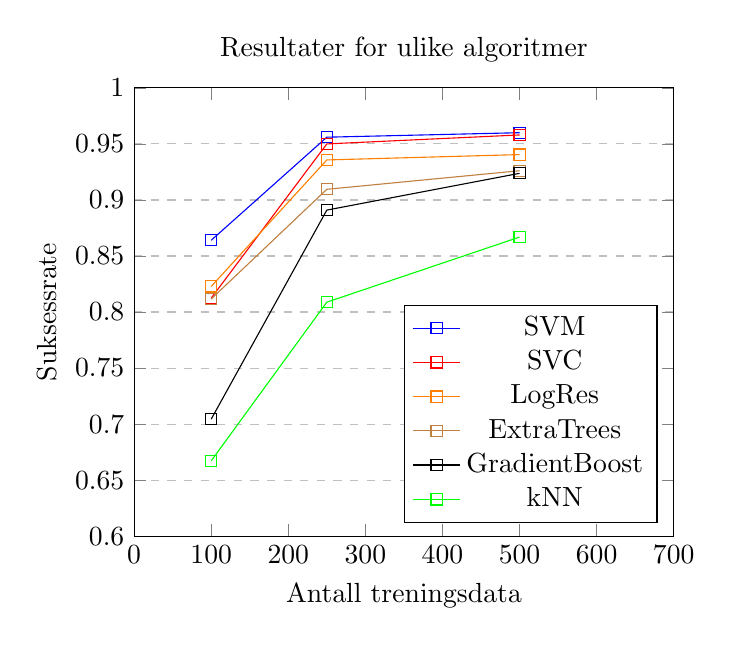
\begin{tikzpicture}
\begin{axis}[
    title={Resultater for ulike algoritmer},
    xlabel={Antall treningsdata},
    ylabel={Suksessrate},
    xmin=0, xmax=700,
    ymin=0.6, ymax=1.0,
    xtick={0,100,200,300,400,500,600,700},
    ytick={0.6,0.65,0.7,0.75,0.8,0.85,0.9,0.95,1.0},
    legend pos=south east,
    ymajorgrids=true,
    grid style=dashed,
]
\addplot[
    color=blue,
    mark=square,
    ]
    coordinates {
    (100,0.864)(250,0.956)(500,0.96)
    };
\addplot[
    color=red,
    mark=square,
    ]
    coordinates {
    (100,0.8124)(250,0.95)(500,0.958)
    };
\addplot[
    color=orange,
    mark=square,
    ]
    coordinates {
    (100,0.8228)(250,0.9357)(500,0.94048)
    };
\addplot[
    color=brown,
    mark=square,
    ]
    coordinates {
    (100,0.8116)(250,0.9095)(500,0.92608)
    };
\addplot[
    color=black,
    mark=square,
    ]
    coordinates {
    (100,0.7044)(250,0.89095)(500,0.92376)
    };
\addplot[
    color=green,
    mark=square,
    ]
    coordinates {
    (100,0.6672)(250,0.8088)(500,0.86688)
    };
    
    \legend{SVM,SVC,LogRes,ExtraTrees,GradientBoost,kNN}
\end{axis}
\end{tikzpicture}
\caption{Resultatsutvikling for et utvalg algoritmer.}
\end{figure}

\subsubsection*{Multimodal interaksjon gjennom tale og gester}
{\color{blue}En argumentasjon for begrenset tale i hjemmet. En løsning på håndtering av multimodal input. Problemer med rejecting-out-of-grammar utterances.}

\subsubsection*{Kombinasjoner}
\begin{table}[h!]
\centering
\begin{tabular}{|| c c c c ||}
\hline
\% Korrekt klassifisering & Algoritme & Antall gester & Treningseksempler/gest \\ [0.5ex] 
 \hline\hline
 94,12 & SVM m/liblinear & 10 & 10 \\ 
 \hline
 92,48 & Logistisk regresjon & 10 & 10 \\ [1ex]
 \hline
 92,4 & SVM m/libsvm & 10 & 10 \\
 \hline
\end{tabular}
\caption{Gjennomsnittsresultater for klassifisering av de samme 10 gestene fra eksperiment 1.}
\label{table:results-foursensors}
\end{table}
{\color{blue}Prosentøkning i eksp.1, hvor stor økning kan man oppnå her?
Langt bedre resultater enn 10 samples av hver over en sensor (.86 .82 .81). Liblinear-algoritmen og logistisk regresjon slår libsvm.  Modellene er trent og testet 100 ganger med tilfeldige utgangspunkt.}
\begin{table}[h!]
\centering
\begin{tabular}{|| c c c c ||}
\hline
\% Korrekt klassifisering & Algoritme & Antall gester & Treningseksempler/gest\\ [0.5ex] 
 \hline\hline
 94,124 & SVM m/libsvm & 42 & 10 \\ 
 \hline
 93,333 & SVM m/liblinear & 42 & 10 \\
 \hline
 92,59 & Logistisk regresjon & 42 & 10 \\ [1ex]
 \hline
\end{tabular}
\caption{Gjennomsnittsresultater for klassifisering av 42 gester.}
\label{table:results-foursensors}
\end{table}
Med kun 10 treningseksempler av hver av de 42 gestene oppnås en suksessrate på 94\%. Modellene er trent og testet 100 ganger med tilfeldige utgangspunkt.

Har fått vist hvordan dimming kan implementeres med en nærhetssensor. Har vist hvordan tale og gester kan benyttes slik at funksjonalitet kun aktiveres dersom begge inputmodaliteter er til stede. Har vist hvordan lysnivåer i hjemmet kan benyttes. 

\subsubsection*{Kontekstdrevet brukergrensesnitt}
Et grafisk brukergrensesnitt, designet delvis etter prinsipper fra grafisk design. En utforskning av et dynamisk brukergrensesnitt. Regeldrevet. Last-value predictor.